\chapter{Methodology}

\section{Participants}

For this study, I recruited six Icelandic speakers who were living in York (UK) at the time the recordings were made.
The methodologies of this research have gained the approval of the Ethics Committee and the subjects received an information sheet and signed a consent form.
Recruitment was done through University channels, the Icelandic Embassy in London and the York Anglo Scandinavian Society.
All the participants were native speakers of Icelandic, above 18 years old and claimed to have normal hearing and speech abilities.
The information on each participant is given in \Cref{t:participants}.
The column labelled ``birthplace'' contains the city or town where the subjects were born; the eventual city or town in parenthesis is the place where they spent most of their life if different from their birthplace.
The last column, ``abroad'', states if the subjects spent more that 6 months outside Iceland.
Participant JR had to be excluded from the analysis since he misunderstood the task, while part of participant SHG's task was lost due to a technical fault in the recording equipment.


\ctable[caption = Information on participants,
label = t:participants,
]{cccclc}{}{
\FL
\textbf{participant} & \textbf{sex}    & \textbf{age} & \textbf{birthplace} & \textbf{languages} & \textbf{abroad} \ML
TT & female & 24 & Reykjavik & English, Danish, German  & Yes \NN
BRS & female & 25 & Hofn      & Danish, English, Spanish & Yes \NN
BTE & female & 27 & Reykjavik & English, Danish          & Yes \NN
JJ & female & 46 & Reykjavik (Kopavogur) & English, Danish          & Yes \NN
SHG & male   & 25 & Selfoss   & English                  & No  \NN
JR & male   & 66 & Reykjavik (York)      & English                  & Yes \LL
}

\section{Materials}

The material used in the task consisted of a list of Icelandic words (the ``target words'') with the following forms: (C)VCC (monosyllabic) and (C)VCCV (bisyllabic).
The list of target words is given in \Cref{a:list}.
The target words were selected so as to control for as many of the following aspects as possible: phonation, manner and place of articulation of consonants following the target vowel; height and frontness of the target vowel; phonation, manner and place of articulation of consonants preceding the target vowel; and height and frontness of the eventual word-final vowel.
Control over these parameters was prioritised according to the order in which they were presented here.
Unfortunately, obtaining a well controlled word list proved to be extremely difficult and several compromises have been made.
%CITE holes and humps papers!

The wordlist contained a total of 58 inflected Icelandic words (only real word forms were used).
These were a mixture of nouns (26), verbs (22), adjectives (8) and adverbs (2).
The 58 words were equally divided in monosyllabic (29) and bisyllabic (29) words.
Of the monosyllabic words, 20 ended with a geminate stop (9 plain geminates and 11 pre-aspirated geminates); 5 with an /NC/ cluster (2 voiced and 3 voiceless nasals); 2 with an /lC/ cluster (one voiced, one voiceless); one word ended with a geminate nasal.
Of the bisyllabic words, 14 had a word-medial geminate stop (8 plain and 6 pre-aspirated); 9 a /NC/ cluster (5 voiced and 4 voiceless); 4 an /lC/ cluster (2 voiced and 2 voiceless); and 2 had an /rC/ cluster (one voiced, one voiceless).



\section{Procedure}

The target words were embedded in the frame sentence \textit{Segðu \_\_ aftur}, `Say \_\_ again.'
This sentence was chosen with the aid of one of the participants so as to control for naturalness, number of syllables and phonetic contexts preceding and following the target word, and phrase stress.
To decision to use a single frame sentence for all the test words was justified by the will of keeping the task as simple as possible.
The participants were asked to read aloud the sentences with the target words shown on a computer screen.
They were advised to speak as naturally as possible, while keeping the same volume and pace.
They did not familiarised themselves with the word list before starting the task.
The decision of not showing the words beforehand was made to reduce the speakers' control over their speech.

The task was presented through the software PyschoPy \citep{peirce2009}, on a Apple MacBook Pro.
Each sentences was shown three times consecutively and the order of appearance was randomised across subjects.
The reading task was self-paced; the participant read a sentence shown on the screen and moved to the next sentence when ready by pressing the space bar.
Four speakers were recorded in a meeting room at a travel agency, while one was recorded at the University of York and the last in his living room, at his house in York.
The only subject who performed the task at the University of York was recorded in a sound-proof studio, using a Beyerdynamic OPUS 54 headset microphone (condenser, cardioid), plugged into a recording station.
The software used for the recording was Adobe Audition, running on a Windows computer.
The other speakers were recorded using the same headset microphone plugged into a Zoom H4n Handy Recorder.
The audio files were encoded using the \texttt{.wav} format at a sampling rate of 44 kHz (16-bit).
Even if the recording conditions differed between participants, the quality of the audio is comparable across files.

\section{Annotation}

\begin{figure}
\centering
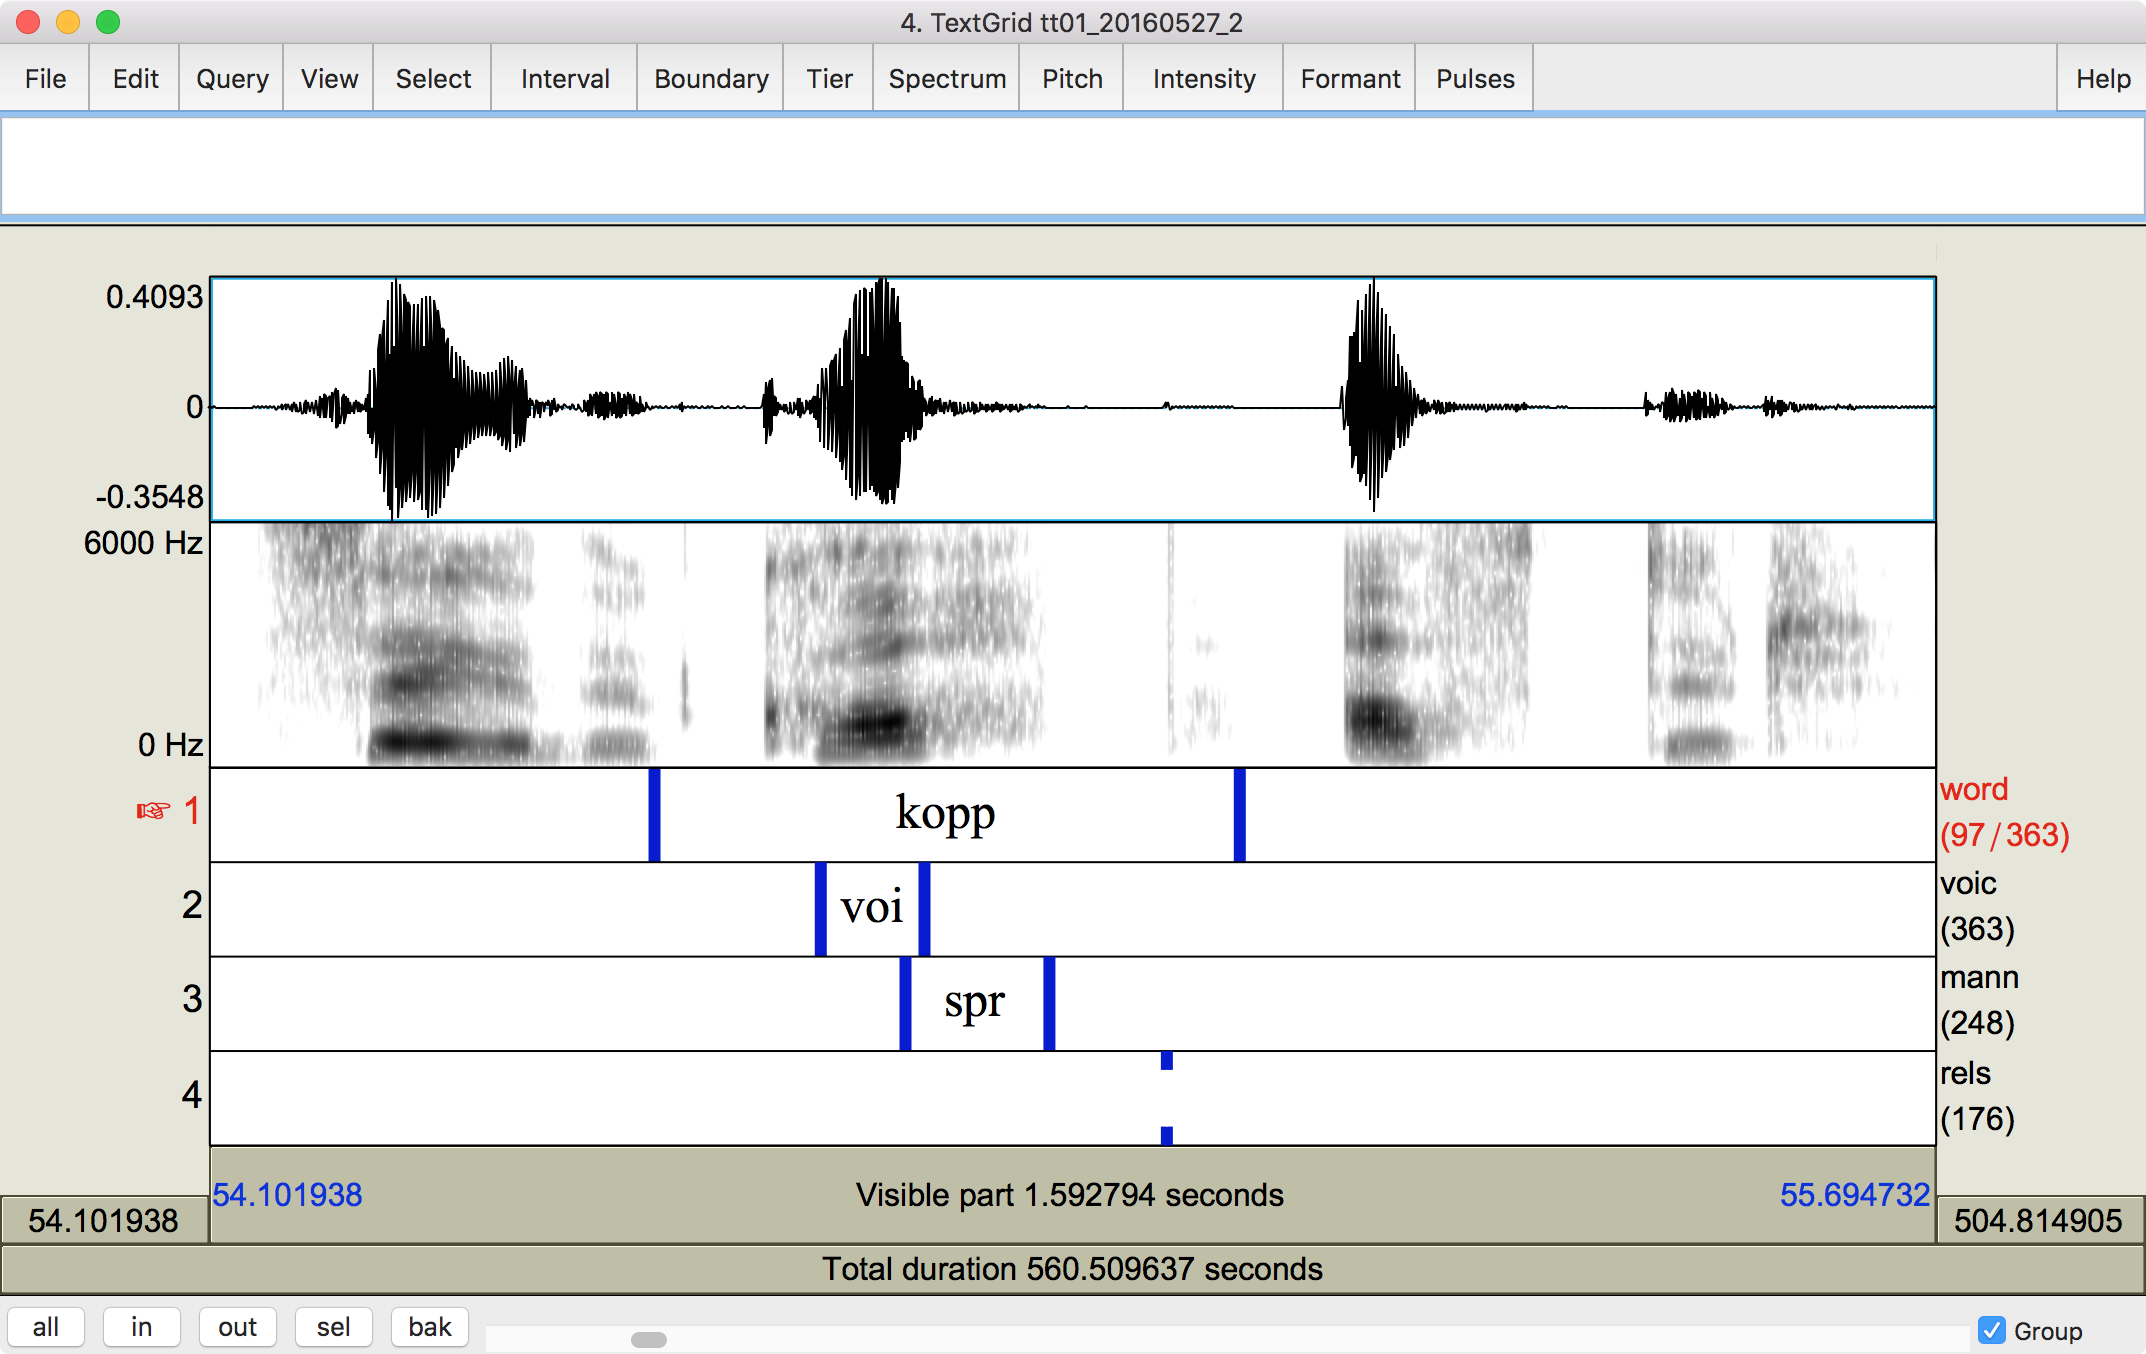
\includegraphics[width=\linewidth]{textgrid}
\caption{Example of the tier structure of the annotation files (PRAAT TextGrids).}
\label{f:textgrid}
\end{figure}

The analysis of the audio file consisted of three phases:
\begin{inparaenum}[(1)]
	\item conversion from stereo to mono,
	\item annotation, and
	\item extraction of measurements.
\end{inparaenum}
I first converted the audio files from stereo to mono, but I did not apply any filter.
During the second phase, I annotated the files in PRAAT \citep{boersma2015} using TextGrid files.
The annotation files have four tiers.
The tiers contain, respectively: 
\begin{inparaenum}[(1)]
	\item the graphemic transcriptions of the target words,
	\item the voiced intervals within the relevant portion of the words, 
	\item the intervals within the words where laryngeal spread, nasality, laterality or rhoticity is present, and
	\item the release of stops.
\end{inparaenum}
\Cref{f:textgrid} shows an example of the TextGrid set-up.

\subsection{Tier 1: words}

The first tier was segmented by target words.
The left boundary of the word was considered to be the off-set of voicing of the final vowel of \textit{segðu}, which preceded the target word.
The right boundary differed between consonant-final and vowel-final words.
In consonant-final words, the right boundary coincided with the end of the friction following the burst of the release, as visible in the waveform and spectrogram.
In vowel-final words, I used different criteria depending on the phonetic realisation.
The right boundary was placed at the off-set of voicing of the word-final vowel if followed by a pause; if the word-final vowel differed from the following and there was no pause, I placed the boundary at the mid-point of the transition between the final vowel and the initial vowel of the following word (\textit{aftur}); if a clear glottal stop separated the target word from the following, the boundary coincided with the on-set of the glottal stop.
In some cases, instead of a glottal stop, creaky voice was visible and the criterion of the transition mid-point was applied.

\subsection{Tier 2: voicing}

The second tier was reserved for the portions of vocal folds vibration (voicing).
The boundaries of the intervals in this tier were placed at the on-set and off-set of voicing around the target vowel.
In words starting with one or more voiced continuant consonants, the portion of voicing of those consonants was excluded from the interval and the left boundary was placed at the beginning of the vowel following the word-initial consonants.

\subsection{Tier 3: glottal spreading}

The third tier was used to annotate glottal spread, nasal airflow, laterality and rhoticity.
Marking the beginning of glottal spread proved to be particularly difficult.
The common realisation of the combination vowel + pre-aspiration is structured as follows: the first portion of the vocalic is accompanied by modal voicing; the glottis starts an abduction gesture while still vibrating the vocal folds (breathy voice); vocal fold vibration stops and voiceless friction remains (at the glottis or at the oral cavity, depending on the vowel).
%ADD glottal picture
As \citet{khan2012} and \citet{nance2013} point out, breathy voice is expected to produce more round-shaped periodic waves.
I took the onset of such more sinusoidal waves to coincide with glottal spread and I marked it as the left boundary of spreading.
However, at times the interpretation of the waveform was not straightforward.
In these cases, I relied on the visual make-up of the spectrogram.
According to \citet{jones2006} (cited in \citet[134]{nance2013}), breathy voice usually correlates with smeared off or totally absent higher formants.
This is due to the presence of high-frequency noise produced by the increased amount of airflow coming from the abducted glottis.
The right boundary was assumed to fall at the end of visible frication noise.

\subsection{Tier 3: nasals, laterals and rhotics}

Following standard practice, I marked the beginning of nasality where a change in the shape of the waveform and in the amplitude of the spectrogram were visible.
I applied the same principle to laterals and rhotics.
I placed the right boundary of these intervals (nasal, lateral, rhotic) depending on the voicing of the segment.
The voiceless nasal, lateral and trill consonants terminate with voiceless friction (nareal, lateral or central, respectively).
The end of friction in these consonants was used as the end of the interval.
In the voiced counterparts of these, the end of voicing coincided with the right boundary.
%ADD manner pictures

\subsection{Tier 4: consonant release}
In tier 4, the release of the stop consonant following the target vowel was marked at the onset of the burst.
If the burst was not visible in the waveform, no release was marked.

\section{Measurements}
%ADD put what you measured
In the third phase, I extracted the durational properties of the annotated intervals through an automated routine.
The routine was run with a PRAAT script, specifically written for this study.
The script with its documentation can be found in \Cref{a:getmeasure}.
The output is a \texttt{.csv} file with the relevant measurements.
The following measures were taken (all measures are in seconds):

\begin{itemize}
\item \textit{Word duration}: the duration of the whole word as annotated on tier 1
\item \textit{Duration of voicing}: the duration of the voicing interval on tier 2
\item \textit{Duration of manner}: the duration of the manner interval on tier 3 (this can be glottal spreading, nasality, laterality or the rhoticity)
\item \textit{Duration of absolute voicing}: this was measured as the duration of the interval between the onset of voicing and the onset of the manner interval, in words containing a pre-aspirated geminate or a sonorant (nasal or liquid); in words with non-aspirated geminates, the duration of absolute voicing is the same as the duration of voicing
\item \textit{Closure duration}: the duration of the stop closure, calculated as the duration of the interval between the off-set of voicing or, if present, manner and the release
\end{itemize}


\section{Statistical analysis}

I performed the statistical analysis using the R programming language \citep{r-core-team2015} in RStudio \citep{rstudio-team2015}.














